\documentclass{article}
\usepackage{bkc}
\usepackage{ccfonts}
\usepackage{tikz-cd}
\usepackage{enumerate}

\setassn{Math 6510 Final Exam}

\usetikzlibrary{decorations.markings,decorations.pathmorphing,matrix,arrows}
\tikzset{middlearrow/.style={
        decoration={markings,
            mark= at position 0.5 with {\arrow{#1}} ,
        },
        postaction={decorate}
    }
}

\newcommand{\im}{\text{im }}

\begin{document}
\begin{problem}{1}{\parindent}
  \vspace*{-\bigskipamount}
  \begin{enumerate}[(a)]
  \item Compute the groups $H_n(X,A)$ when $X$ is $S^2$ of $S^1\times
    S^1$ and $A$ is a finite set of points.
  \item Compute $H_n(X,A)$ and $H_n(X,B)$ where $X$ is a closed
    orientable surface of genus 2 and $A$ and $B$ are the circles
    shown in the figure below.
    \begin{center}
      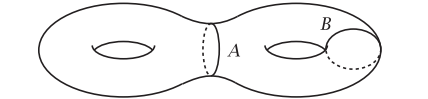
\includegraphics[scale=.5]{torus.png}
    \end{center}
  \end{enumerate}
\end{problem}
\begin{solution}{\parindent}
  \begin{enumerate}[(a)]
  \item We begin with the former. Let $X = S^2$ and $A =
    \{a_1,\ldots,a_n\}$ be a finite set of points. If $n = 0$ then
    trivially $H_n(X,A) = H_n(X)$. for the non-trivial case we observe
    that $(X,A)$ is a good pair because we can surround each of the
    points $a_i \in A$ by a small disk in $X$ which deformation
    retracts onto $a_i$ via the straight line homotopy. We then note
    that there are no $k$-cells in $X$ for $k > 2$ and consequently
    $H_n(X,A) = 0$ for $n > 2$. For $n \leq 2$ we can consider the
    long exact sequence of the pair
    \begin{center}
      \begin{tikzcd}
        \cdots \arrow{r} & H_2(A) \arrow{r} & H_2(X) \arrow{r} &
        H_2(X,A) \arrow{r} & H_1(A) \arrow{r} & \cdots
      \end{tikzcd}
    \end{center}
    Then we note that $A$ is a discrete set of points and consequently
    $H_n(A) = 0$ for $n > 0$ and moreover $H_2(X) = \Z$. This reduces
    the above to
    \begin{center}
      \begin{tikzcd}
        0 \arrow{r} & \Z \arrow{r} & H_2(X,A) \arrow{r} & 0
      \end{tikzcd}
    \end{center}
    Then exactness of the sequence implies that $H_2(X,A) \cong
    \Z$. Looking further down the sequence we see
    \begin{center}
      \begin{tikzcd}
        \cdots \arrow{r} & H_1(A) \arrow{r} & H_1(X) \arrow{r} &
        H_1(X,A) \arrow{r} & H_0(A) \arrow{r} & \cdots
      \end{tikzcd}
    \end{center}
    This time we have $H_1(A) = H_1(X) = 0$, $H_0(A) =
    \bigoplus_{i=1}^{n} \Z$ (one generator for each of the $a_i$) and
    $H_0(X) = \Z$. Thus, the above becomes
    \begin{center}
      \begin{tikzcd}
        0 \arrow{r} & 0 \arrow{r} & H_1(X,A) \arrow{r} &
        \bigoplus_{i=1}^{n} \Z \arrow{r}{p} & \Z
      \end{tikzcd}
    \end{center}
    Exactness implies $H_1(X,A) = \ker p$. We know that homomorphisms
    must fix the identity and consequently must send only one
    generator of the product to $1 \in \Z$. This means that $\ker p =
    \bigoplus_{i=1}^{n-1} \Z$ and $H_1(X,A) = \bigoplus_{i=1}^{n-1}
    \Z$. Lastly, we have that
    \begin{center}
      \begin{tikzcd}
        \cdots \arrow{r} & H_0(A) \arrow{r} & H_0(X) \arrow{r} &
        H_0(X,A) \arrow{r} & 0
      \end{tikzcd}
    \end{center}
    By previous arguments these give
    \begin{center}
      \begin{tikzcd}
        \cdots \arrow{r} & \bigoplus_{i=1}^{n}\Z \arrow{r} & \Z \arrow{r} &
        H_0(X,A) \arrow{r} & 0
      \end{tikzcd}
    \end{center}
    In particular the end of the sequence implies that $H_0(X,A) =
    0$. This gives
    \[
    H_k(X,A) =
    \begin{cases}
      0 & k = 0 \\
      \bigoplus_{i=1}^{n-1} \Z & k = 1 \\
      \Z & k = 2 \\
      0 & k > 2
    \end{cases}
    \]

    When $X = S^1 \times S^1$ we proceed much in the same way as
    previously. The pair $(X,A)$ is still a good pair for the same
    reason as before. for $H_2(X,A)$ we note that $H_2(A) = 0$,
    $H_2(X) = \Z$ and $H_1(A) = 0$ so we get the sequence
    \begin{center}
      \begin{tikzcd}
        \cdots \arrow{r} & 0 \arrow{r} & \Z \arrow{r} & H_2(X,A)
        \arrow{r} & 0
      \end{tikzcd}
    \end{center}
    Which implies that $H_2(X,A) = \Z$. Proceeding down the sequence
    we recall that $H_1(X) = \Z \times \Z$ so the sequence at this
    level (terminated with a 0) becomes
    \begin{center}
      \begin{tikzcd}
        0 \arrow{r} & \Z\oplus \Z \arrow{r} & H_1(X,A)
        \arrow{r} & \bigoplus_{i=1}^n \Z \arrow{r} & 0
      \end{tikzcd}
    \end{center}
    We then apply the Splitting Lemma to conclude that
    \[
    H_1(X,A) \cong (\Z \oplus \Z) \oplus \bigoplus_{i=1}^n \Z \cong
    \bigoplus_{i=1}^{n+1} \Z
    \]
    Finally, for $H_0(X,A)$ we have the sequence
    \begin{center}
      \begin{tikzcd}
        0 \arrow{r} & \bigoplus_{i=1}^n \Z \arrow{r} & \Z
        \arrow{r} & H_0(X,A) \arrow{r} & 0
      \end{tikzcd}
    \end{center}
    Which immediately implies $H_0(X,A) = 0$. Aggregating these
    computations we have
    \[
    H_k(X,A) =
    \begin{cases}
      0 & k = 0\\
      \bigoplus_{i=1}^{n+1} \Z & k = 1 \\
      \Z & k =2 \\
      0 & k > 2
    \end{cases}
    \]
    Again, we remark that if $A = \emptyset$ then $H_k(X,A) = H_k(X)$.
  \item We begin with $H_n(X,A)$. First recall that $H_n(X,A) =
    \tilde{H}_n(X,A)$ because $(X,A)$ is a good pair. But $X/A$ is a
    wedge of two tori. If we embed $X/A$ into $\R^3$ in the usual way
    and consider an open neighborhood that deformation retracts onto
    each of the $S^1 \times S^1$ factors, respectively, then we can
    use the Mayer-Vietoris sequence to compute the homology. Indeed,
    if we let $U \supset S^1\times S^1$ and $V \supset S^1\times S^1$
    be such neighborhoods then we have
    \begin{center}
      \begin{tikzcd}
        \cdots \arrow{r} & \tilde{H}_n(U \cap V) \arrow{r} &
        \tilde{H}_n(U) \oplus \tilde{H}_n(V) \arrow{r} &
        \tilde{H}_n(X) \arrow{r} & \tilde{H}_{n-1}(U \cap V) \arrow{r} &
        \cdots
      \end{tikzcd}
    \end{center}
    We then note that $U \cap V$ deformation retracts to a point and
    therefore has the homology of a point. This reduces the sequence
    for each $n$ to
    \begin{center}
      \begin{tikzcd}
        0 \arrow{r} & \tilde{H}_n(S^1\times S^1) \oplus
        \tilde{H}_n(S^1\times S^1) \arrow{r} & \tilde{H}_n(X/A)
        \arrow{r} & 0
      \end{tikzcd}
    \end{center}
    Exactness then states precisely that 
    \[
    \tilde{H}_n(X/A) = \tilde{H}_n(S^1\times S^1) \oplus
    \tilde{H}_n(S^1\times S^1)
    \]
    In particular we see that
    \[
    H_n(X,A) = \tilde{H}_n(X/A) =
    \begin{cases}
      0 & n = 0 \\
      \bigoplus_{i=1}^4 \Z & n=1 \\
      \Z \oplus \Z & n=2 \\
      0 & n \geq 3
    \end{cases}
    \]

    If we identify $X$ with the octagon (having the usual
    identifications), we can see that collapsing $B$ to a point
    removes one of the generators and we see that the quotient space
    is homeomorphic to $S^1 \times S^1/\{x_0,x_1\}$ where
    $\{x_0,x_1\}$ result from cancelling the other generator for that
    loop. We can then apply the previous part of this question to see that
    \[
    H_0(X,B) =
    \begin{cases}
      0 & n = 0 \\
      \Z \oplus \Z \oplus \Z & n =1 \\
      \Z & n=2 \\
      0 &
    \end{cases}
    \]
  \end{enumerate}
\end{solution}

\begin{problem}{2}{\parindent}
  Show that $\tilde{H}_n(X) \cong \tilde{H}_{n+1}(SX)$ for all $n$,
  where $SX$ is the suspension of $X$. More generally, thinking of
  $SX$ as the union of two cones $CX$ with their bases identified,
  compute the reduced homology of the union of $n$ cones $CX$ with
  their bases identified.
\end{problem}
\begin{solution}{\parindent}
  For the fist part, we will use the Mayer-Vietoris sequence. Indeed,
  we take the cover to be $A = p(X \times [0,1/2 + \epsilon])$ and $B
  = p(X \times [1/2-\epsilon, 1]$ where $p$ is the quotient map for
  the suspension. It is clear that $A \cap B$ deformation retracts
  onto $X$, so the Mayer-Vietoris sequence in reduced homology becomes
  \begin{center}
    \begin{tikzcd}
      \cdots \arrow{r} & \tilde{H}_{n+1}(A \cap B) \arrow{r} &
      \tilde{H}_{n+1}(A) \oplus \tilde{H}_{n+1}(B) \arrow{r} &
      \tilde{H}_{n+1}(SX) \arrow{r} & \tilde{H}_{n}(A \cap B) \arrow{r}
      & \cdots
    \end{tikzcd}
  \end{center}
  We then note that $A$ and $B$ deformation retract to the cone $CX$
  on $X$, which is homotopy equivalent to a point, and consequently
  has the homology of a point. Thus, the above sequence becomes
  \begin{center}
    \begin{tikzcd}
      0 \oplus 0 \arrow{r} & \tilde{H}_{n+1}(SX) \arrow{r} &
      \tilde{H}_{n}(X) \arrow{r} & 0\oplus 0
    \end{tikzcd}
  \end{center}
  Exactness of the sequence gives $\tilde{H}_{n+1}(SX) \cong
  \tilde{H}_{n}(X)$ as desired.

  For the union of $n$ cones we proceed by induction on the number of
  cones. Let $C^{n}X$ be the union of $n$ cones on $X$We will show
  that
  \[
  \tilde{H}_{n+1}(C^nX) = \bigoplus_{i=1}^{n-1} \tilde{H}_{n}(X)
  \]
  We have just done the base case in the previous part. We can choose
  a cover of $C^{n}X$ by $C^{n-1}X$ and $CX$ then the Mayer-Vietoris
  sequence becomes
  \begin{center}
    \begin{tikzcd}
      0 \arrow{r} & \tilde{H}_{n+1}(CX) \oplus
      \tilde{H}_{n+1}(C^{n-1}X) \arrow{r} & \tilde{H}_{n+1}(C^nX)
      \arrow{r} & \tilde{H}_{n}(X) \arrow{r} & 0
    \end{tikzcd}
  \end{center}
  By the splitting lemma we have that
  \[
  \tilde{H}_{n+1}(C^nX) \cong \tilde{H}_{n}(X) \oplus
  \left(\bigoplus_{i=1}^{n-2} \tilde{H}_{n}(X)\right) \cong
  \bigoplus_{i=1}^{n-1} \tilde{H}_{n}(X)
  \]
\end{solution}

\begin{problem}{3}{\parindent}
  As on page 136 of the book, the local homology groups of a space $X$
  at a point $x \in X$ are defined to be the relative homology groups
  $H_n(X,X-\{x\})$. Let $X$ be the cone on the 1-skeleton of
  $\Delta^3$, the union of all the line segments joining the six edges
  of $\Delta^3$ to the barycenter of $\Delta^3$
  \begin{enumerate}[(a)]
  \item Compute the local homology groups $H_n(X,X-\{x\})$ for all $x
    \in X$.
  \item Define $\partial X$ to be the subset of $X$ consisting of
    points $x$ such that the local homology groups $H_n(X,X-\{x\})$
    are zero for all $n$. Compute the local homology groups
    $H_n(\partial X,\partial X - \{x\})$ for all $x \in \partial X$.
  \item Use these calculuations to determine which subsets $A \subset
    X$ have the property that $f(A) \subset A$ for all homeomorphisms
    $f:X \to X$.
  \end{enumerate}
\end{problem}
\begin{solution}{\parindent}
  \begin{enumerate}
  \item We begin by noting that there are five cases depending on
    where $x$ lies inside of $C\Delta^3$. We handle them in sequence:
    \begin{enumerate}
    \item Suppose that $x$ is a vertex in $\Delta^3$. We see that
      locally we have a star-shaped nieghborhood $U$ corresponding to
      the three faces and the edge leading to the barycenter. This
      neighborhood deformation retracts to a point (first project down
      to the plane so we have the wedge of four line segments, and
      then retract each of the segments). Consequently, each
      (sufficiently) small neighborhood of $x$ has the homotopy type
      of a point. We then recall that homology is a homotopy invariant
      and so $\tilde{H}_n(U,U - \{x\}) = 0$.
    \item The next case is the ``distinguished vertex'' that is the
      barycenter. Note that if we remove the barycenter, the resulting
      space $C\Delta^3 - \{x\}$ deformation retracts to $\Delta^3_1$,
      the 1-skeleton of $\Delta^3$. We can then compute the homology
      groups based on the $k$-skeletons of $\Delta^3$. Indeed we have
      the chain complex
      \begin{center}
        \begin{tikzcd}
          \cdots \arrow{r} & 0 \arrow{r} & \bigoplus_{i=1}^6 \Z
          \arrow{r}{\partial_1} & \bigoplus_{i=1}^4 \Z
          \arrow{r}{\partial_0} & 0
        \end{tikzcd}
      \end{center}
      It is clear from this that $\tilde{H}_1(X) = \bigoplus_{i=1}^4
      \Z$ and $\tilde{H}_n(X) = 0$ otherwise. This implies that
      \[
      H_n(U, U-\{x\}) \cong \tilde{H}_{n-1}(\Delta^3_1) =
      \begin{cases}
        \bigoplus_{i=1}^3 \Z & n = 2 \\
        0 & \text{otherwise}
      \end{cases}
      \]
    \item Now we look at the interior points of $C\Delta^3$. Suppose
      that $x$ lies on an edge in $\Delta^3$. Then a neighborhood $U$
      of $x$ will be contractible and thus we have $\tilde{H}_n(U -
      \{x\}) = 0$ and consequently $H_n(U, U - \{x\}) = 0$.
    \item If $x$ lies on an edge connecting to the barycenter, then
      the situation is a bit different. We see that $x$ will intersect
      three faces in this case. 
    \item The last case is clear. If $x$ is in the interior of the
      space then any neighborhood of $x$ is homeomorphic to a disk in
      $\R^2$ and so the homology is 0 for all $n$. Thus, we have a
      situation very similar to the barycenter. After removing $x$ we
      have a space that deformation retracts onto tetrahedron and so
      the homology must be the same as the barycenter for this
      reason. Thus we have that
      \[
      H_n(U, U-\{x\}) \cong \tilde{H}_{n-1}(\Delta^3_1) =
      \begin{cases}
        \bigoplus_{i=1}^3 \Z & n = 2 \\
        0 & \text{else}
      \end{cases}
      \]
    \end{enumerate}
    again.
  \item In this case, we simply have the exterior of $\Delta^3$ (if we
    aggregate the results from the previous part.) There are only a
    few changes when we compute the local homology in $\partial
    X$. The change occurs when we consider the vertices of
    $\Delta^3$. In this case we note that a vertex on an edge must
    have a neighborhood that deformation retracts onto $S^2 \wedge
    S^2$ so that
    \[
    H_n(X,X - \{x\} \cong \tilde{H}_n(S^2\wedge S^2 \cong
    \tilde{H}_2(S^2)\oplus \tilde{H}_2(S^2)
    \]
    The others are unchanged.
  \item Suppose that $f$ is a homeomorphism of $X$. Then we must have
    that
    \[
    H_n(X, X - \{x\}) \cong H_n(X, X - \{f(x)\})
    \]
    for each $n$. Thus, we can restrict $f$ to a homeomorphism on
    $\Delta_1^3$. In particular, see from part (b) that $f$ must map
    vertices to vertices, and so it must permute the vertices. Also,
    we see that $f$ must fix the barycenter of $X$. Finally, we notice
    that $f$ must also fix the edges within $X$ and so if we let
    $v_0,\ldots,v_3$ denote the vertices $b$ the barycenter
    $e_1,\ldots,e_n$ the edges then we have that the invariant sets
    under any homeomorphism must be obtained from the following:
    \begin{enumerate}
    \item $\{v_0,\ldots,v_3$
    \item $\{b\}$
    \item $\{\Delta_1^3\}$
    \item $\{e_1,\ldots,e_n$
    \item $X = C\Delta^3$
    \end{enumerate}
    under the set theoretic operations of union, intersection and set
    subtraction.
  \end{enumerate}
\end{solution}

\begin{problem}{4}{\parindent}
  On the first exam,there was a problem asking for the calculation of
  the fundamental froup of the CW complex obtained from a cube $I^3$
  by identifying opposite faces by a one-quarter twist. Now compute
  the homology groups of this complex, without using the general fact
  that $H_1$ is the abelianization of $\pi_1$.
\end{problem}
\begin{solution}{\parindent}
  See the attached diagram.
\end{solution}

\begin{problem}{5}{\parindent}
  Two problems to solve using Mayer-Vietoris sequences:
  \begin{enumerate}[(a)]
  \item Show that a closed nonorientable surface, or more generally
    any finite CW complex $X$ for which $H_1(X)$ contains torsion (an
    element of finite order), cannot be embedded as a subspace fo
    $\R^3$ in such a way that it has a neighborhood which is a mapping
    cylinder of a map from a closed orientable surface to $X$.
  \item The closed orientable surgace $M_g$ of genus $g$ embedded in
    $\R^3$ in the standard way bounds a compact region $R$. Two copies
    of $R$ glued together by the identity map between their boundaries
    form a closed 3-manifold $X$. Compute the homology groups of $X$.
  \end{enumerate}
\end{problem}
\begin{solution}{\parindent}
  \begin{enumerate}
  \item Suppose towards a contradiction that $X$ could be embedded in
    $\R^3$. Then the mapping cylinder neighborhood $M$ of $f(X)$
    deformation retracts onto $f(X)$. We then consider the
    Mayer-Vietoris sequence for the pair $U = \overline{M}$ and $V =
    \overline{\R^3 - M}$. Then observe that the intersection $U \cap B
    = \partial M$. The sequence in reduced homology becomes
    \begin{center}
      \begin{tikzcd}
        \tilde{H}_2(\R^3) \arrow{r} & \tilde{H}_1(\partial M)
        \arrow{r} & \tilde{H}_1(U) \oplus \tilde{H}_1(V) \arrow{r} &
        \tilde{H}_1(\R^3)
      \end{tikzcd}
    \end{center}
    We then note that $\partial M \cong M_g$ the surface of genus $g$
    and as a result we see that the above actually gives
    \begin{center}
      \begin{tikzcd}
        0 \arrow{r} & \Z^{2g} \arrow{r} & \tilde{H}_1(f(X)) \oplus
        \tilde{H}_1(V) \arrow{r} & \tilde{H}_1(\R^3)
      \end{tikzcd}
    \end{center}
    and by exactness we see that $\Z^{2g} \cong \tilde{H}_1(f(X))
    \oplus \tilde{H}_1(V)$. But we assumed that $H_1(X)$ had torsion
    which is a contradiction because $\Z^{2g}$ is torsion-free.
  \item the Mayer-Vietoris sequence says that
    \begin{center}
      \begin{tikzcd}
        \cdots \arrow{r} & H_n(M_g) \arrow{r} & H_n(R) \oplus H_n(R)
        \arrow{r} & H_n(X) \arrow{r} & H_{n-1}(M_g) \arrow{r} & \cdots
      \end{tikzcd}
    \end{center}
    We then note that $R$ deformation retracts onto $\vee_{i=1}^g S^1$
    in the usual way. Thus, $H_0(R) \cong \bigoplus_{i=1}^g
    \Z$. As a result we see that
    \begin{center}
      \begin{tikzcd}
        0 \arrow{r} & H_n(X) \arrow{r} & H_{n-1}(M_g) \arrow{r} & 0
      \end{tikzcd}
    \end{center}
    Thus we get that
    \[
    H_n(X) =
    \begin{cases}
      \Z & n=0 \\
      \bigoplus_{i=1}^g \Z & n=1 \\
      \bigoplus_{i=1}^g \Z \cong H_1(M_g) & n=2 \\
      \Z \cong H_2(M_g) & n = 3 \\
      0 & n \geq 4
    \end{cases}
    \]
    where the $n=1$ case follows because the image of $M_g$ in the
    induced map is the diagonal in $H_1(R) \oplus H_1(R)$.
  \end{enumerate}
\end{solution}

\begin{problem}{6}{\parindent}
  The mapping cylinders of a sequence of maps
  \begin{center}
    \begin{tikzcd}
      X_1 \arrow{r}{f_1} & X_2 \arrow{r}{f_2} & X_3 \arrow{r} & \cdots
    \end{tikzcd}
  \end{center}
  can be joined together to form the \emph{mapping telescope} $T$
  which is the quotient space of $\coprod_{n=1}^\infty (X_n \times I)$
  under the identifications $(x_n,1) \sim (f(x_n),0)$ for all $x_n \in
  X_n$, $n = 1,2,\cdots$.
  \begin{enumerate}[(a)]
  \item Let each $X_n$ be $S^1$ and let $f_n: S^1 \to S^1$ be a
    basepoint-preserving map of degree $n$. Compute $\pi_1(T)$ and
    $H_i(T)$ for all $i$. Also, show that $\pi_i(T) = 0$ for all $i >
    1$ using a compactness argument and the fact that part of a
    mapping telescope $T$ between $X_1$ and $X_n$ deformation retracts
    onto $X_n$.
  \item For $k > 1$ let each $X_n$ be $S^k$ and let $f_n: S^k \to S^k$
    be a basepoint preserving map of degree $n$. Compute $\pi_1(T)$
    and $H_i(T)$ for all $i$.
  \end{enumerate}
\end{problem}
\begin{solution}{\parindent}
  \begin{enumerate}[(a)]
  \item We will compute $\pi_1(T)$ by applying van Kampen's
    theorem. Each of the open sets in the cover will be a neighborhood
    $A_n$ of one of the $S^1 \times I$ factors in $T$. Then each of
    the $A_n$ is path-connected and open.  Moreover, each of the $A_n
    \cap A_{m} \cap A_\ell = \emptyset$. Consequently, we have a
    surjective homomorphism $\Phi: \ast_{k=1}^\infty \Z \to
    \pi_1(T)$. To compute the elements in $\ker\Phi$ we note that
    $f_n$ has degree $n$ for each $n$ and therefore is $n$ times the
    generator for $\pi_1(S^1)$. This yields the following presentation
    for the fundamental group
    \[
    \pi_1(T) \cong \lbrace \sum_{n=1}^\infty a_n \mid na_n =
    (n+1)a_{n+1}\rbrace
    \]
    We then remark that this implies that each of the $a_n$ can be
    written in terms of $a_1$. This gives an isomorphism $\pi_1(T) \to
    \bigoplus_{n=1}^\infty \Z/n\Z$ by sending $a_n \to na_1$. The
    reason that this group is free abelian is that each of the
    generators commute with one another because the union is
    disjoint. Consequently, $H_1(T)$ as the abelianization of
    $\pi_1(T)$ is also $\bigoplus_{n=1}^\infty \Z/n\Z$.
  \item In this case van Kampen's theorem gives us that $\pi_1(T) =
    0$. The reason is that we can set the $A_n = S^k \times I$ which
    is simply connected and therefore there is a surjective
    homomorphism from $0 \to \pi_1(T)$. For the homology groups, we
    will do a limiting process. Let $T_n$ be the product
    $\coprod_{n=1}^\infty (S^k \times I)$ modulo the same relations as
    $T$. In this case we consider the Mayer-Vietoris sequence
    $(T_n,S^k)$ so that we have
    \begin{center}
      \begin{tikzcd}
        \cdots \arrow{r} & H_n(S^k \cap T^{n-1}) \arrow{r} & H_n(S^k)
        \oplus H_n(T^{n-1}) \arrow{r} & H_n(T^n) \arrow{r} &
        H_{n-1}(S^k \cap T^{n-1} \arrow{r} & \cdots
      \end{tikzcd}
    \end{center}
    We will show by induction that
    \[
    H_n(T^n) =
    \begin{cases}
      \bigoplus_{i=1}^n \Z/n\Z & n = k \\
      0 & \text{otherwise}
    \end{cases}
    \]
    Indeed, note that the sequence becomes
    \begin{center}
      \begin{tikzcd}
        H_n(S^k) \arrow{r} & H_n(S^k) \oplus H_n(T^{n-1}) \arrow{r} &
        H_n(T^n) \arrow{r} & H_{n-1}(S^k \cap T^{n-1})
      \end{tikzcd}
    \end{center}
    When $n = k$ we get
    \begin{center}
      \begin{tikzcd}
        \Z \arrow{r} & \Z \oplus \left(\bigoplus_{i=1}^{n-1} \Z/n\Z\right)
        \arrow{r} & H_n(T^n) \arrow{r} & 0
      \end{tikzcd}
    \end{center}
    then we use degree to see that the induced map sends the generator
    of $\Z$ to $n\Z$ implying that the induced map forces
    \[
    H_n(T^n) \cong \Z/n\Z \oplus \left(\bigoplus_{i=1}^{n-1}
      \Z/n\Z\right) \cong \bigoplus_{i=1}^{n} \Z/n\Z
    \]
    By the induction hypothesis. If $n \neq k$ then $H_n(S^k) = 0$
    implies that $H_n(T^n) = 0$ as well.
  \end{enumerate}
\end{solution}
\end{document}
